\subsection{CVSS-Vektor Selektion} \label{subsec:projektbericht-loesungsweg-cvss-selection}

Mit dem Format aus Kapitel \ref{subsec:projektbericht-loesungsweg-cvss-source-management} werden ab Generation 3 des Vulnerability Monitorings der {\metaeffekt} ALLE Vektoren zu den gefundenen Schwachstellen mit in das Inventar der Komponenten aufgenommen.
Generation 2 dieses Systems hat diese Multiplizität der Vektoren einfach übergangen.
Da die Auswahl der effektiven Vektoren als Nebeneffekt des zuständigen Codes durch ein \qt{First-Come-First-Serve}-Verfahren realisiert war, wurde eine bewusste Entscheidung der Kunden von Anfang an ausgeschlossen.
Um zu jedem Zeitpunkt die genaue Quelle eines Vektors nachvollziehbar zu halten, werden bei dem neuen System zunächst alle Vektoren über den Prozessverlauf aggregiert und erst in den Schritten ausgewertet werden, in denen sie interpretiert werden müssen.
Die Funktionsweise der CVSS-Vektor-Selektion wird in diesem Kapitel erklärt.

Vor Beginn ist konzeptionell erneut zu betonen, dass die Auswahl der, von den vorhergegangenen Prozessschritten angesammelten, Vektoren wirklich erst ab den Schritten geschieht, in denen sie auf egal welcher Art und Weise dargestellt oder für weitere Berechnungen benötigt werden.
Die Selektion bezieht sich immer auf die Vektoren einer einzigen, vollständigen Schwachstelle.
Dieser Prozess wird in zwei Teile geteilt, da für einige Use-Cases bereits das Zwischenergebnis von Interesse ist.

Ein Schritt, der vor der Auswahl stattfinden muss, ist es, erst die relevanten Vektoren einer Schwachstelle zu sammeln.
Hierfür gibt es einige Fälle die beachtet werden müssen:
Natürlich werden alle Vektoren, die direkt auf der Schwachstelle sind, direkt hinzugefügt.
Einige Vektoren werden nicht von der Schwachstelle selbst, sondern von referenzierten Security Advisories beigetragen, also müssen auch diese eingesammelt werden.
Doch nicht immer sind alle Vektoren anwendbar, zum Beispiel bei Vektoren von Microsoft gibt es Bedingungen, wann ein Vektor anwendbar ist.
Diese Bedingungen müssen hier erst ausgewertet werden, wodurch Vektoren eventuell herausgefiltert werden.
Zudem kann es sein, dass ein projektinternes Bewertungsteam eigene Vektoren für eine Schwachstelle vergeben hat, diese müssen natürlich auch berücksichtigt werden.

Um die Einordnung des Themas zu vereinfachen, wird dieser Prozess beispielhaft in Schaubild \ref{fig:cvss-selection-process-collection} mit dem Betriebssystem \qt{Windows 10 Pro} mit frei erdachten, jedoch realistischen Schwachstellen, Security Advisories und Vektor-Quellen durchgeführt.
\ifshortenedReport
Dieses betroffene Betriebssystem durchläuft als Komponente die Inventory Enrichment Pipeline, und bekommt damit die gefundenen Schwachstellen und Security Advisories angehängt.
\else
Dieses betroffene Betriebssystem durchläuft als Komponente die Inventory Enrichment Pipeline, wie in Kapitel \ref{subsec:projektbericht-grundlagen-vulnerability-monitoring} beschrieben, und bekommt damit die gefundenen Schwachstellen und Security Advisories angehängt.
\fi
Nicht nur die Schwachstelle und die Security Advisories wurden mit CVSS-Vektoren versehen, sondern gab es auch mehrere Vektor-Modifikationen von manuellen Bewertungen als \qt{Assessment}-Vektoren.
Das Beispiel wird in Kapitel \ref{subsubsec:projektbericht-loesungsweg-cvss-selection-example} mit der Selektion der Vektoren weitergeführt.

\begin{figure}[htbp] % here, top, bottom, separate page
    \centering
    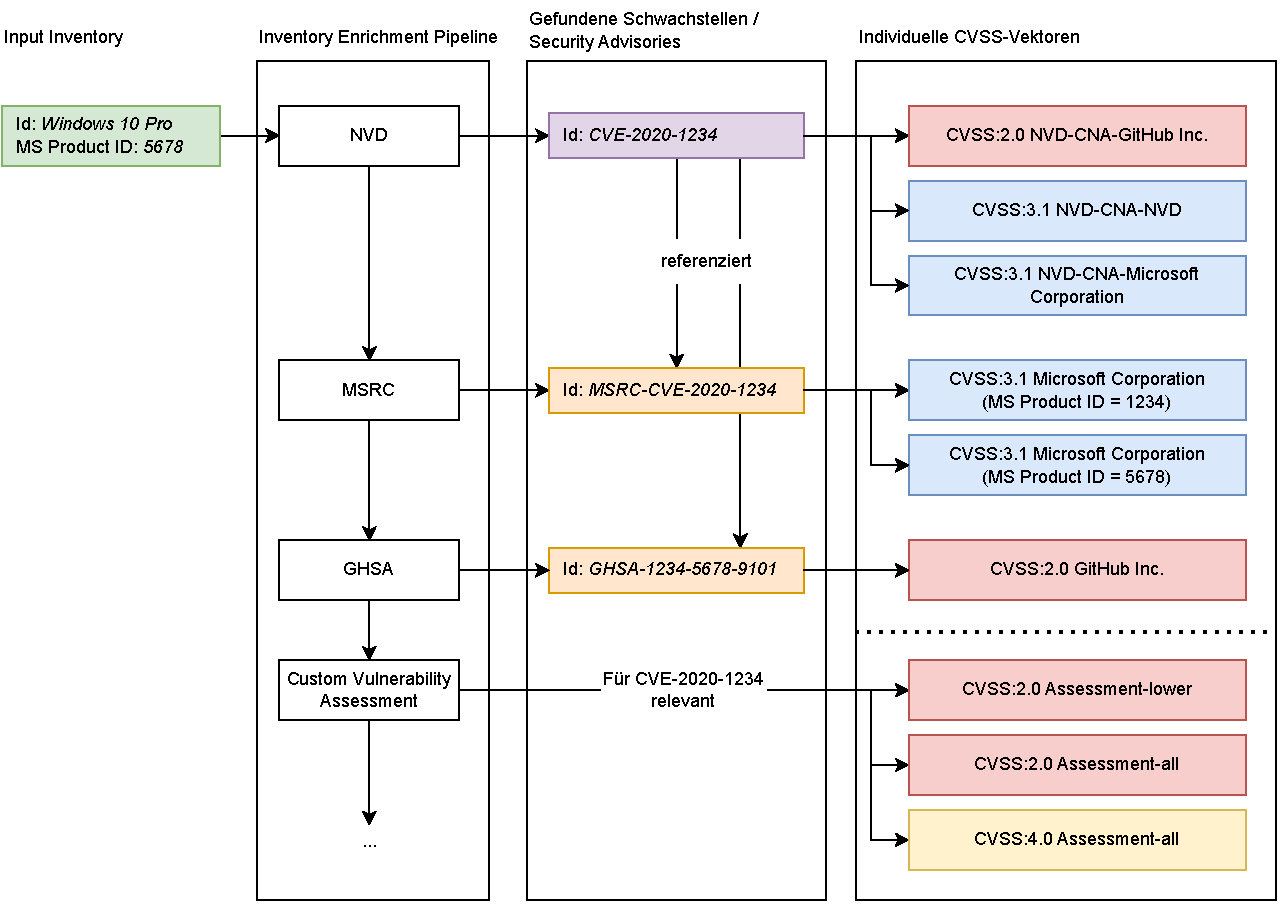
\includegraphics[width=1\textwidth, keepaspectratio]{res/grafiken/cvss-selection-process-collection}
    \caption{Beispiel: Initialer Zuordnungs- und Sammelungsschritt für Schwachstelldaten und CVSS-Vektoren}
    \label{fig:cvss-selection-process-collection}
\end{figure}

Nachdem alle Vektoren angesammelt wurden, kann die Selektion gestartet werden, die, wie bereits erklärt, in zwei Teile aufgeteilt ist.
Wichtig ist zudem, dass der Auswahlprozess in der Realität zwei Mal stattfinden muss, einmal für einen \qt{initial} und einen \qt{context} Selektor.
Der Grund dafür ist, dass es für Kunden wichtig ist, die Nachvollziehbarkeit, welcher Vektor und Score von den externen Datenquellen gekommen ist und wie sie diesen durch ihre \qt{assessment}-Vektormodifikationen verändert haben.

\begin{enumerate}
    \item
    Nutze einen Selektor, um aus allen aggregierten Vektoren eine reduzierte Menge zu bilden, die pro Version nur einen Vektor enthält.
    Diese Vektoren werden für Radardiagramme als Übersicht und zur Aufschlüsselung der unterschiedlichen Einschätzungen und Interpretationen zwischen den Versionen verwendet.
    Dieser Schritt macht den Hauptteil der Berechnungslogik aus, da er hoch anpassbar sein soll.
    \item
    Eine weitere Regel wird dann auf diesem ersten Ergebnis benutzt, um zwischen den unterschiedlichen Versionen zu entscheiden und einen als effektiven Vektor für die Schwachstelle zu bestimmen.
    Dieser wird für die Repräsentation der Schwachstelle in weiteren Diagrammen und Tabellen verwendet, da eine Differenzierung zwischen Versionen auf solch einem höheren Betrachtungslevel nicht sinnvoll oder relevant ist.
\end{enumerate}

\subsubsection{Schritt 1: Selektionsregeln} \label{subsubsec:projektbericht-loesungsweg-cvss-selection-rules-1}

Allgemein ist der Selektionsschritt in drei Abschnitte aufteilbar.
Der erste sucht in potenziell mehreren Schritten, definiert durch gekapselte Regeln, Vektoren aus der aggregierten Menge an Vektoren heraus und kombiniert diese auf eine definierbare Weise.
Die darauffolgenden beiden Schritte dienen zur Auswertung des Ergebnisvektors, um diesen eventuell noch einmal zu manipulieren oder etwa in bestimmten Situationen gar keinen zurückzugeben.

Ein Auszug der relevanten Klasse mit ihren Attributen, die für die Selektion aus Schritt 1 zuständig sind, kann in Listing \ref{lst:cvss-selector-class-attributes} gefunden werden.
Der volle Quellcode mit der Logik kann auf dem \href{https://github.com/org-metaeffekt/metaeffekt-core/blob/24a26dd37ab6f9087e2fdc1b338857b404fa835e/libraries/ae-security/src/main/java/org/metaeffekt/core/security/cvss/processor/CvssSelector.java}{[öffentlichen Repository]} gefunden werden.
Eine weitere Anforderung für das dahinterliegende Datenmodell der Selektoren ist es, komplett als JSON-Objekt serialisierbar zu sein, aus dem dann wieder eine identische Java-Objektstruktur aufgebaut werden kann.
Im Quellcode werden darum einige Konvertierungsmethoden zur Verfügung gestellt.

% basicstyle=\tiny
\begin{lstlisting}[language=Java, label={lst:cvss-selector-class-attributes}, caption={CVSS-Selektor Klassen}, basicstyle=\scriptsize]
public class CvssSelector {
    // Die Attribute werden in diesen Unterkapiteln erklaert.
    List<CvssRule> rules; // 1.1
    List<SelectorStatsEvaluator> statsEvaluatorActions; // 1.2
    List<SelectorVectorEvaluator> selectorVectorEvaluators; // 1.3

    public static class CvssRule {
        SourceSelector sourceSelector;
        MergingMethod mergingMethod;
        List<SelectorStatsCollector> statsCollectors;
        List<SelectorVectorEvaluator> vectorEvaluators;
    }
    public static class SourceSelector {
        List<SourceSelectorEntry> preferredSources;
    }
    public static class SourceSelectorEntry {
        List<SourceSelectorEntryEntry<CvssEntity>> hostingEntities;
        List<SourceSelectorEntryEntry<CvssEntity>> issuingEntities;
        List<SourceSelectorEntryEntry<CvssIssuingEntityRole>> issuingEntityRoles;
    }
    public static class SourceSelectorEntryEntry<T extends CvssSource.EntityNameProvider> {
        T value;
        boolean inverted;
    }
    public static class SelectorStatsCollector {
        String attributeName;
        StatsCollectorProvider provider;
        StatsCollectorSetType setType;
    }
    public static class SelectorVectorEvaluator {
        // operations are combined using AND
        // individual operations can be inverted by setting value to true
        Map<VectorEvaluatorOperation, Boolean> operations;
        EvaluatorAction action;
    }
    public static class SelectorStatsEvaluator {
        String attributeName;
        StatsEvaluatorOperation comparator;
        EvaluatorAction action;
        Integer comparisonValue;
    }
    public enum MergingMethod {
        ALL, LOWER, HIGHER, OVERWRITE
    }
    public enum StatsCollectorProvider {
        PRESENCE, ABSENCE, APPLIED_PARTS_COUNT
    }
    public enum StatsCollectorSetType {
        ADD, SUBTRACT, SET, MAX, MIN
    }
    public enum StatsEvaluatorOperation {
        EQUAL, SMALLER, SMALLER_OR_EQUAL, GREATER, GREATER_OR_EQUAL
    }
    public enum VectorEvaluatorOperation {
        IS_NULL, IS_BASE_FULLY_DEFINED, IS_BASE_PARTIALLY_DEFINED, IS_ENVIRONMENTAL_PARTIALLY_DEFINED, IS_TEMPORAL_PARTIALLY_DEFINED, IS_THREAT_PARTIALLY_DEFINED
    }
    public enum EvaluatorAction {
        FAIL, RETURN_NULL, SKIP, RETURN_PREVIOUS
    }
}
\end{lstlisting}

\paragraph{Schritt 1.1: Regeln zur Vektor-Selektion und -Kombination} \label{par:projektbericht-loesungsweg-cvss-selection-rules-1-1}

Zur Selektion (und Kombination) der effektiven Vektoren werden von einem Benutzer eine Menge an Regeln definiert.
Diese legen je fest, welchen Vektor sie auswählen, wie mit Ergebnissen umgegangen werden soll und ob nutzerdefinierte Variablen modifiziert werden sollen.
Zunächst werden die im Code in der Klasse \code{SourceSelector} als \code{SourceSelectorEntry} benannten Regeleinträge erklärt.
Diese Klassen verwendet die Vektor-Quellennotation, wie in Kapitel \ref{subsec:projektbericht-loesungsweg-cvss-source-management} aufgeführt, zur Eingrenzung des Vektors, der ausgewählt werden soll.
Die einzelnen Einträge erlauben es, Hosting- und Issuing-Entities und eine Issuing Role anzugeben, mit Sonderwerten von \qt{*} für das matchen von beliebigen, aber nicht-leeren Werten und \qt{null}, um einen leeren Wert zu verlangen, die gegen jeden Vektor der Eingangsvektoren gehalten werden.
Das Ergebnis kann optional durch einen weiteren Parameter bei jeder Auswertung invertiert werden, um komplexere Abfragen zu erlauben.
Der erste erfolgreiche Eintrag, der einen Vektor findet, wird an die obere Ebene zurückgegeben, was die Definition von fallback-Strategien ermöglicht.

% Horizontal is this instance, vertical is the parameter.
% |       | ANY | value | null |
% |-------|-----|-------|------|
% | ANY   | Y   | Y     | Y    |
% | value | Y   | ==    | N    |
% | null  | N   | N     | Y    |

Wenn von den Selektoren ein Vektor zurückgegeben wurde, wird über eine \code{MergingMethod} definiert, auf welche Art dieser auf den der vorherigen Regel angewendet werden sollte.
Die häufigste Methode ist \code{ALL}, welche einfach alle Metriken, die von dem gefundenen Vektor definiert sind, auf dem vorherigen setzt.
Weitere Optionen sind \code{HIGHER} und \code{LOWER}, welche Metriken nur dann anwenden, wenn der daraus entstehende Vektor einen gleichen oder höheren/niedrigeren Score, je nach Methode, hervorbringt.
Dies ist nützlich bei Assessment-Vektoren (vom Bewertungsteam ausgestellten), die global auf ein gesamtes Inventar zur begründeten Herunterstufung der Schwachstellen angewendet werden sollen, wie, wenn die Applikation vom Internet komplett abgeschirmt ist oder eine andere Metrik für einen Kontext nicht relevant ist.
Die letzte Option ist \code{OVERWRITE}, welche einfach vollständig den vorherigen Vektor durch den neuen ersetzt.

Beim Anwenden dieser Vektoren werden über die \code{SelectorStatsCollector} verschiedene ganzzahlig numerische Statistiken in benutzerdefinierte Variablen für die \qt{Statistics Evaluators} in Schritt 1.2 getrackt.
Beispielsweise kann ein \qt{Statistics Collector} erstellt werden, der trackt, ob ein Vektor von einer gewissen Regel gefunden wurde (präsenz-Check), oder wie viele Metriken von diesem angewandt wurden (also ob der Vektor modifiziert wurde), was bei den Methoden \code{HIGHER} und \code{LOWER} nützlich sein kann.
Diese Variablen werden bis zum Schritt 1.2 gespeichert, bei dem sie ausgewertet werden können.

Zuletzt können pro Regel noch Checks mit \code{SelectorVectorEvaluator} durchgeführt werden.
Diese können Aktionen über \code{EvaluatorAction} auslösen, wie:
den Prozess komplett scheitern zu lassen, einen leeren Vektor zurückzugeben, diese eine Regel zu überspringen oder an der vorherigen Regel abzubrechen.
Diese Checks können optional invertiert werden.

\paragraph{Schritt 1.2: Statistics Evaluators (Statistik-Auswerter)}

Nun, da in Schritt 1.1 (Unterkapitel von \ref{par:projektbericht-loesungsweg-cvss-selection-rules-1-1}) von den Regeln ein einziger, kombinierter Vektor gebaut wurde, können optional einige der \qt{Statistics Collectors} über die \code{SelectorStatsEvaluator} ausgewertet werden.
Hier werden die typischen numerischen Vergleichsmethoden wie größer, kleiner, gleich, und so weiter zur Verfügung gestellt, um auch hier die Aktionen aus \code{EvaluatorAction} ausführen zu können.

\paragraph{Schritt 1.3: Vector Evaluators}

Abschließende Checks auf dem Ergebnisvektor können wieder über die \code{SelectorVectorEvaluator} durchgeführt werden und über \code{EvaluatorAction} Aktionen auslösen, wie bereits in Schritt 1.1 erklärt.

Dieser komplette Prozess wird bei der {\metaeffekt} je einmal pro Vektor-Version (2.0, 3.1, 4.0) mit jeweils zwei Selektoren (initial, context) durchgeführt und ergibt damit kombinatorisch eine Menge von bis zu sechs Vektoren.

\subsubsection{Schritt 2: Versions-Selektionsregeln} \label{subsubsec:projektbericht-loesungsweg-cvss-selection-rules-2}

Dieser Schritt ist wesentlich einfacher als Schritt 1, da er nur noch angeben muss, von welcher Vektor-Version der effektive Vektor gewählt werden soll.
Die verfügbaren Werte sind in Listing \ref{lst:cvss-selector-version-selector} zu sehen.
Es gibt zwei Kategorien, einmal auf die Vektor-Version (mit latest, oldest und den einzelnen version 2, 3 und 4) und einmal auf die Werte der Scores (höchster, niedrigster) bezogenen.
Die zwei Meistverwendeten sind \code{LATEST}, gefolgt von \code{HIGHEST}.

\begin{lstlisting}[language=Java, label={lst:cvss-selector-version-selector}, caption={Gültige Werte für die Versions-Selektion}]
public enum CvssScoreVersionSelectionPolicy {
    HIGHEST, LOWEST, LATEST, OLDEST, V2, V3, V4
}
\end{lstlisting}

Nach Anwenden dieser beiden Schritte ist die Selektion vollständig durchgeführt.
Im folgenden Abschnitt wird diser Prozess anhand eines Beispiels demonstriert.

\subsubsection{Beispiel zur Vektor-Selektion} \label{subsubsec:projektbericht-loesungsweg-cvss-selection-example}

Das Beispiel, begonnen unter Kapitel \ref{subsec:projektbericht-loesungsweg-cvss-selection} im Schaubild \ref{fig:cvss-selection-process-collection}, wird hier mit den aggregierten Vektoren fortgeführt.
Um die Selektion durchzuführen werden die beiden folgenden Selektoren für initial und context verwendet, die dank einer \code{CvssSelector.explain()}-Methode als menschenlesbarer Text dargestellt werden können.
Diese gezeigten und verwendeten Selektoren sind auch die, die als Standard-Werte im Produktionscode\footnote{\href{https://github.com/org-metaeffekt/metaeffekt-core/blob/1f0a1f6ac5e8343e10ea182794faf534bdfb3310/libraries/ae-inventory-processor/src/main/java/org/metaeffekt/core/inventory/processor/report/configuration/CentralSecurityPolicyConfiguration.java\#L568}{\texttt{https://github.com/org-metaeffekt/metaeffekt-core/blob/...}}} eingetragen sind.

\paragraph{Beispiel, CVSS-Selektor \qt{initial}} \label{par:projektbericht-loesungsweg-cvss-selection-example-selector-initial}

Dies ist der Selektor, der im Folgenden als \qt{initial} bezeichnet wird.

\noindent The CVSS Selector contains 1 rule that will be applied in the following order:
\begin{enumerate}[noitemsep]
    \setlist{nolistsep}
    \item The first matching vector is selected: [NVD-CNA-NVD], [Microsoft Corporation-*-*], [NVD-CNA-Microsoft Corporation], [GitHub, Inc.-*-*], [NVD-CNA-GitHub, Inc.], [NVD-*-*], [CERT-SEI-*-*], [not:Assessment-*-*]. From the selected vector, all vector components are applied to the resulting vector.
\end{enumerate}

\paragraph{Beispiel, CVSS-Selektor \qt{context}} \label{par:projektbericht-loesungsweg-cvss-selection-example-selector-context}

Dies ist der Selektor, der im Folgenden als \qt{context} bezeichnet wird.
Er enthält die Basisregel des \qt{initial}-Selektors, und wird durch Regeln bezüglich der Assessment-Vektoren ergänzt, um eine kontextualisierte Sicht zu ermöglichen.

\noindent The CVSS Selector contains 4 rules that will be applied in the following order:
\begin{enumerate}[noitemsep]
    \setlist{nolistsep}
    \item The first matching vector is selected: [NVD-CNA-NVD], [Microsoft Corporation-*-*], [NVD-CNA-Microsoft Corporation], [GitHub, Inc.-*-*], [NVD-CNA-GitHub, Inc.], [NVD-*-*], [CERT-SEI-*-*], [not:Assessment-*-*]. From the selected vector, all vector components are applied to the resulting vector.
    \item If present, the [Assessment-*-all] vector is selected. From the selected vector, all vector components are applied to the resulting vector. The following 1 statistics collector will also be applied to the selected vector:
    \begin{itemize}[noitemsep]
        \item If a vector is returned from the selection, 1 is added to the stats collector attribute [assessment].
    \end{itemize}
    \item If present, the [Assessment-*-lower] vector is selected. From the selected vector, only vector components that lead to a lower or equal score on the resulting vector are applied. The following 1 statistics collector will also be applied to the selected vector:
    \begin{itemize}[noitemsep]
        \item If a vector is returned from the selection, 1 is added to the stats collector attribute [assessment].
    \end{itemize}
    \item If present, the [Assessment-*-higher] vector is selected. From the selected vector, only vector components that lead to a higher or equal score on the resulting vector are applied. The following 1 statistics collector will also be applied to the selected vector:
    \begin{itemize}[noitemsep]
        \item If a vector is returned from the selection, 1 is added to the stats collector attribute [assessment].
    \end{itemize}
\end{enumerate}

\noindent After finishing the CVSS selection, 1 statistics evaluator will be applied to the resulting vector:
\begin{itemize}[noitemsep]
    \setlist{nolistsep}
    \item If the stats collector attribute [assessment] is equal to 0, then no vector is returned.
\end{itemize}
Additionally, 1 vector evaluator will be applied to the resulting vector:
\begin{itemize}[noitemsep]
    \setlist{nolistsep}
    \item If the resulting vector is not base fully defined, then no vector is returned.
\end{itemize}

\paragraph{Beispiel, Schritt 1: Aggregieren der Vektoren} \label{par:projektbericht-loesungsweg-cvss-selection-example-step-1}

Dieser Abschnitt bezieht sich auf Schaubild \ref{fig:cvss-selection-process-selection-1}.

Zunächst muss, als Eingabe für die Selektionsschritte, eine Menge an Vektoren gesammelt werden.
Da sich dieses Beispiel auf die Schwachstelle \qt{CVE-2020-1234} aus dem vorhergegangenen Beispiel bezieht, werden auf jeden Fall alle Vektoren der Schwachstelle selbst und der referenzierten manuellen Bewertungen (\qt{Assessments}) aufgenommen.
Bedingte Vektoren müssen nun noch auf ihre Bedingung geprüft werden:
Microsoft ordnet pro Produkt in ihren Datensätzen nur einen Vektor zu, darum wird der Vektor mit der Beziehung zu \qt{MS Product ID 1234} herausgefiltert, da die Id der verwendeten Komponente \qt{5678} darauf nicht referenziert wird.

\begin{figure}[htbp] % here, top, bottom, separate page
    \centering
    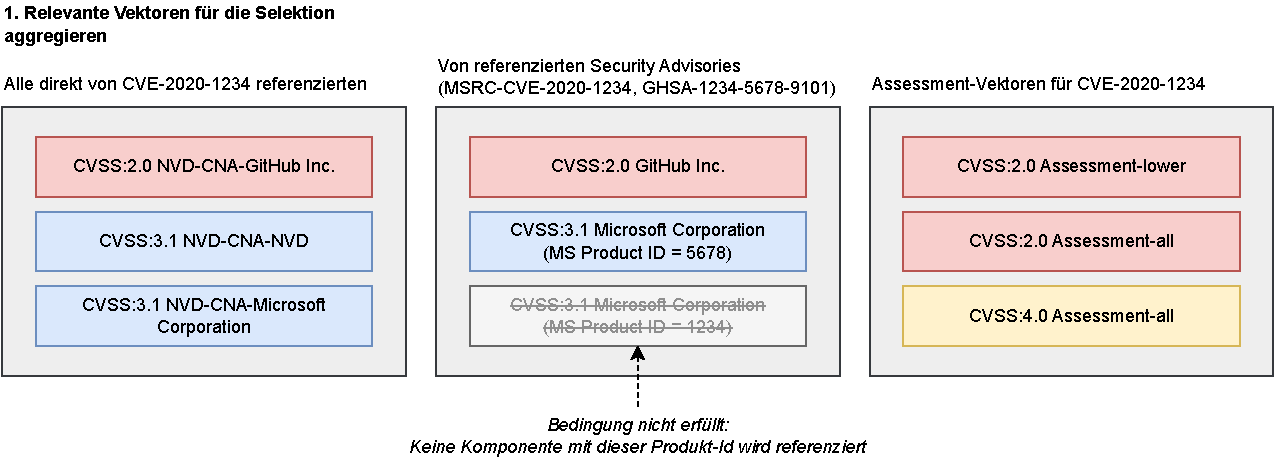
\includegraphics[width=1\textwidth, keepaspectratio]{res/grafiken/cvss-selection-process-selection-1}
    \caption{Aggregierung der CVSS-Vektoren}
    \label{fig:cvss-selection-process-selection-1}
\end{figure}

\paragraph{Beispiel, Schritt 2: Anwenden der CVSS-Selektoren} \label{par:projektbericht-loesungsweg-cvss-selection-example-step-2}

Dieser Abschnitt bezieht sich auf die Schaubilder \ref{fig:cvss-selection-process-selection-2} und \ref{fig:cvss-selection-process-selection-3}.

\begin{figure}[htbp] % here, top, bottom, separate page
    \centering
    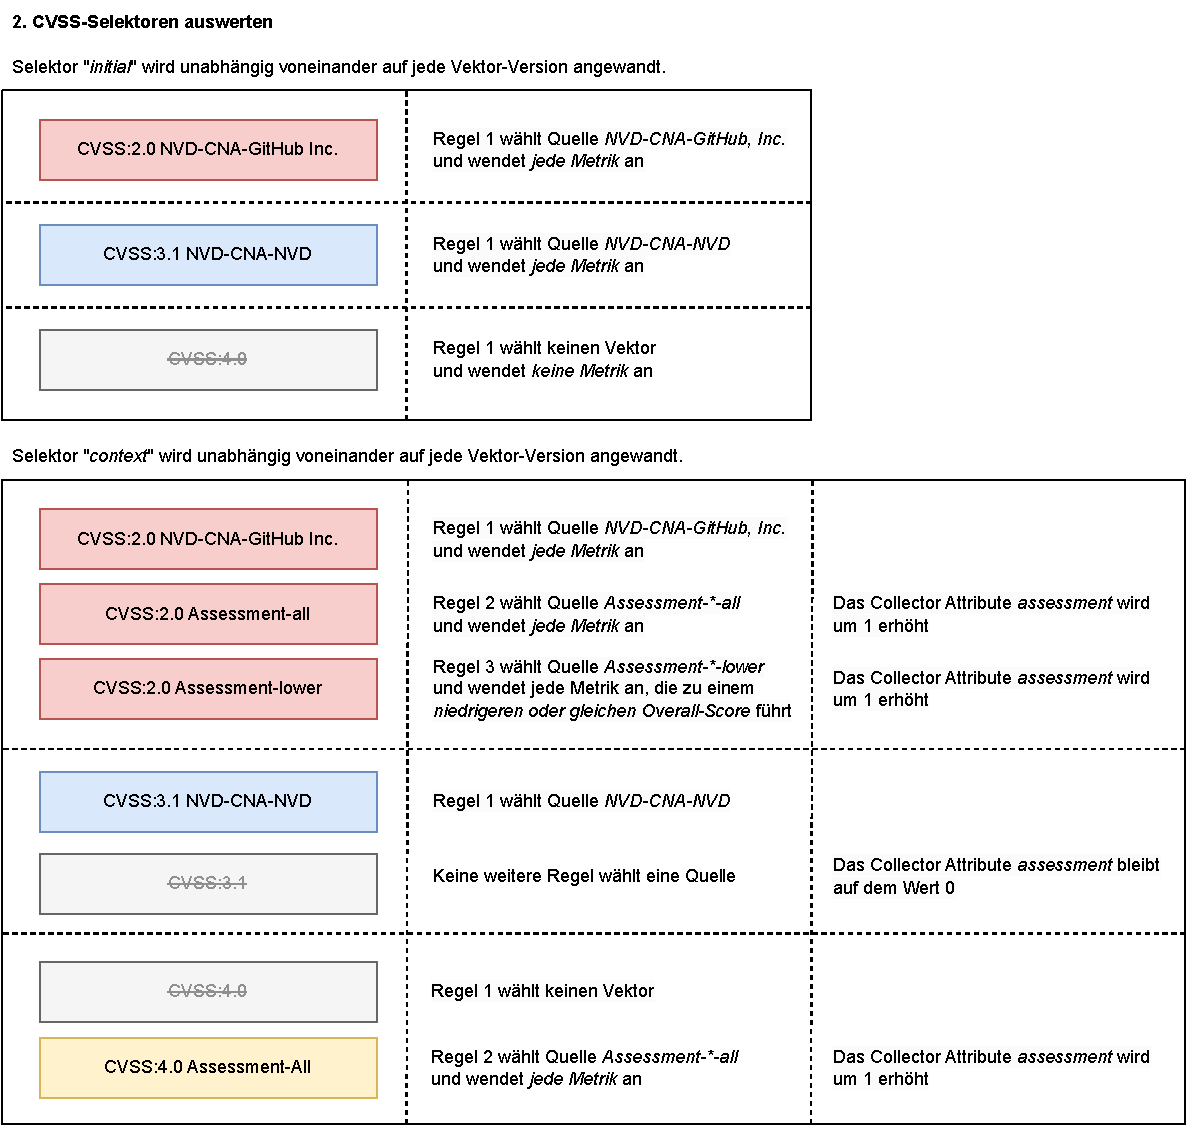
\includegraphics[width=1\textwidth, keepaspectratio]{res/grafiken/cvss-selection-process-selection-2}
    \caption{Auswerten der CVSS-Selektoren}
    \label{fig:cvss-selection-process-selection-2}
\end{figure}

\begin{figure}[htbp] % here, top, bottom, separate page
    \centering
    \includegraphics[width=1\textwidth, keepaspectratio]{res/grafiken/cvss-selection-process-selection-3}
    \caption{Ergebnisse der CVSS-Selektion}
    \label{fig:cvss-selection-process-selection-3}
\end{figure}

Nun können die Selektoren auf die Vektor-Menge angewendet werden.
Im Fall des \qt{initial}-Selektors wird einfach die erste zutreffende Quelle aus der Liste in Regel 1 gewählt.
Außer bei CVSS:4.0 (keine nicht-Assessment-Vektoren) wird hier immer genau ein Vektor zurückgegeben.

Bei dem \qt{context}-Selektor werden genau dieselben initialen Vektoren zunächst ausgewählt, bei CVSS:2.0 wird allerdings noch von den anderen Regeln 2 und 3 ein Vektor gefunden und entsprechend den Regeln angewandt (alle Metriken, nur \qt{lower}).
Bei CVSS:4.0 wird sogar nur durch einen Assessment-Vektor eine Kontribution gemacht, nicht durch etwa Regel 1.
Hierbei merkt sich das System auch, ob mindestens ein Assessment-Vektor vorgekommen ist, was nur bei CVSS:3.1 nicht der Fall war.
Das bedeutet, wie in Schaubild \ref{fig:cvss-selection-process-selection-3} zu sehen, dass zwar für CVSS:2.0 ein kombinierter und für CVSS:4.0 der Assessment-Vektor gewählt werden konnten, aber für CVSS:3.1 durch den Statistics Evaluator, der das \qt{assessment} Attribut überprüft, kein Vektor zurückgegeben wurde.

\paragraph{Beispiel, Schritt 3: Anwenden der Versions-Selektion} \label{par:projektbericht-loesungsweg-cvss-selection-example-step-4}

Dieser Abschnitt bezieht sich auf Schaubild \ref{fig:cvss-selection-process-selection-4}.

Nun können die verbleibenden Vektoren auf einen einzigen je \qt{initial} und \qt{context} durch den Versions-Seletor reduziert werden.
Hier wird einfach \code{LATEST} angewandt, das heißt, die höchste Versionszahl gewinnt.
Diese Vektoren können nun für weitere Zwecke verwendet werden.

\begin{figure}[htbp] % here, top, bottom, separate page
    \centering
    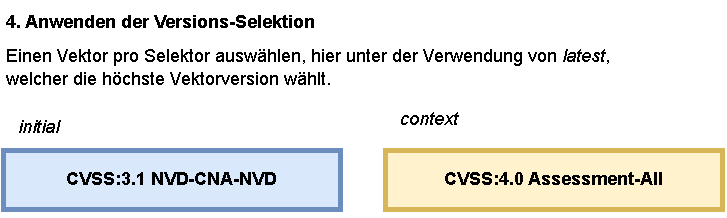
\includegraphics[width=0.7\textwidth, keepaspectratio]{res/grafiken/cvss-selection-process-selection-4}
    \caption{Anwenden der Versions-Selektion}
    \label{fig:cvss-selection-process-selection-4}
\end{figure}
